\documentclass[border=10pt]{article}
%%%<
\usepackage{verbatim}
%%%>
\usepackage{pgfplots}
\pgfplotsset{width=7cm,compat=1.8}
\usepgfplotslibrary{ternary}

\begin{document}
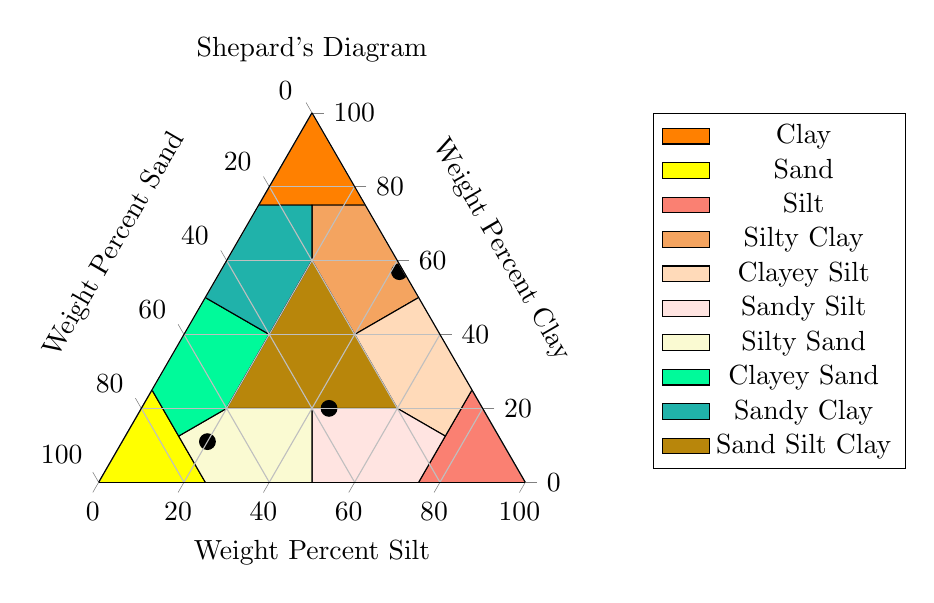
\begin{tikzpicture}

\definecolor{sand}{rgb}{1,1,0}
\definecolor{clay}{rgb}{1,.5,0}
\definecolor{silt}{rgb}{ 0.980392, 0.501961, 0.447059}
\definecolor{sand_silt_clay}{rgb}{0.721569, 0.52549, 0.0431373}
\definecolor{sandy_silt}{rgb}{1, 0.894118, 0.882353}
\definecolor{sandy_clay}{rgb}{0.12549, 0.698039, 0.666667}
\definecolor{silty_clay}{rgb}{ 0.956863, 0.643137, 0.376471}
\definecolor{silty_sand}{rgb}{ 0.980392, 0.980392, 0.823529}
\definecolor{clayey_sand}{rgb}{0, 0.980392, 0.603922}
\definecolor{clayey_silt}{rgb}{ 1, 0.854902, 0.72549}

0.803922 0.360784 0.360784
\begin{ternaryaxis}[
	title=Shepard's Diagram,
	xlabel=Weight Percent Clay,
	ylabel=Weight Percent Sand,
	zlabel=Weight Percent Silt,
	label style=sloped,
	area style,
        legend style={at={(1.3,1)}}
]
	\addplot3 [fill = clay] table {
	A B C
	1 0 0
	0.75 0.25 0
	0.75 0 0.25
	};
	\addlegendentry{Clay}

        \addplot3 [fill = sand] table {
	A B C
	0 1 0
	0.25 0.75  0
	 0 0.75 0.25
	};
	\addlegendentry{Sand}

\addplot3  [fill = silt] table {
	A B C
	0 0 1
	0.25 0 0.75  
	 0  0.25 0.75
	};
	\addlegendentry{Silt}

\addplot3 [fill = silty_clay] table {
	A B C
	.5 0  0.5
	0.4 0.2  0.4  
	 0.6 0.2  0.2
        .75 .125  .125
        .75 0       .25
	};
	\addlegendentry{Silty Clay}

\addplot3 [fill =clayey_silt] table {
	A B C
	.5 0  0.5
	0.4 0.2  0.4  
	 0.2 0.2  0.6
        .125 .125  .75
        .25 0       .75
	};
	\addlegendentry{Clayey Silt}

\addplot3 [fill = sandy_silt]table {
	A B C
	0 .5 0.5
	0.2 0.4 0.4  
	 0.2  0.2 0.6
        .125 .125 .75
        0    .25   .75
	};
	\addlegendentry{Sandy Silt}

\addplot3 [fill = silty_sand] table {
	A B C
	0 .5 0.5
	0.2 0.4 0.4  
	 0.2  0.6 0.2
        .125 .75 .125
        0    .75   .25
	};
	\addlegendentry{Silty Sand}

\addplot3 [fill = clayey_sand] table {
	A B C
	.5 0.5 0  
	0.4  0.4 0.2    
	 0.2 0.6  0.2
        .125 .75  .125
        .25 .75 0       
	};
	\addlegendentry{Clayey Sand}


\addplot3 [fill = sandy_clay] table {
	A B C
	.5 0.5 0  
	0.4  0.4 0.2    
	 0.6 0.2  0.2
        .75 .125  .125
        .75 .25 0       
	};
	\addlegendentry{Sandy Clay}


\addplot3 [fill = sand_silt_clay] table {
	A B C
	.20 .20 0.6
	0.2 0.6 0.2  
	 0.6  0.2 0.2
	};
	\addlegendentry{Sand Silt Clay}


	\node[inner sep=2pt,circle,draw,fill=black] at (axis cs:0.57,0.01,0.42) {};

\node[inner sep=2pt,circle,draw,fill=black] at (axis cs:0.11,0.69,0.2) {};

\node[inner sep=2pt,circle,draw,fill=black] at (axis cs:0.2,0.36,0.44) {};
	
\end{ternaryaxis}
\end{tikzpicture}
\end{document}
